\item {\bf [5 pts.] Continental Geotherms} \\
    Consider the structure below of a series of anticlines and synclines.
    Imagine this package of layered rocks were sediments with alternating
    quartzite and shale layers.
    \begin{figure}[hbt]
        \centering
        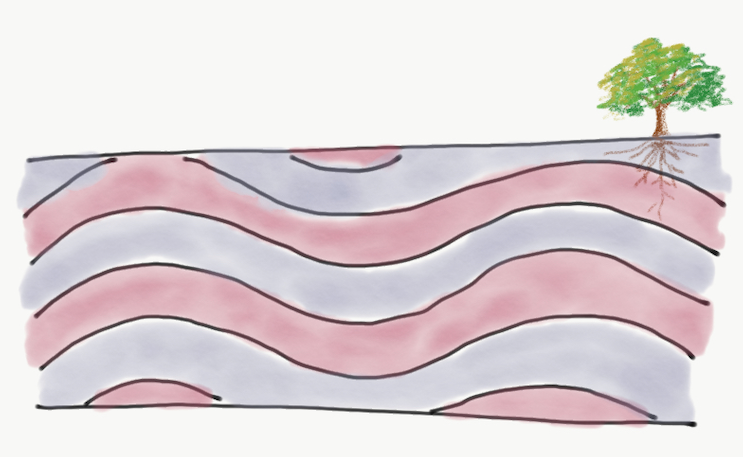
\includegraphics[width=0.75\textwidth]{figures/anticlines.png}
        \caption{A series of anticlines and synclines.}
        \label{fig:structure}
    \end{figure}

    \begin{enumerate}
        \item What are reasonable values for the thermal conductivities of the
        two layers?

        \item Assuming heat flow at the base of the stuctures are constant
        along the bottom plane, draw flow lines which indicate the direction for
        the heat flow associated with these structures.

        \item Now draw isolines for the flow of heat associated with these
        structures.  Remember, temperature at the surface is constant.  As a
        result you may have to make adjustments to your flow lines from the
        previous part.

        \item If we were to collect temperaturatures in two boreholes, one at
        the hinge of the antilcline and another at the hinge of the syncline,
        what would the temperature versus depth look like for the two respective
        holes?  Remember the variations in thermal conductivity.

        \item What would vertical heat flow look like as a profile across this
        cross section?
    \end{enumerate}
